\documentclass[12pt]{article}

\usepackage{sbc-template}
\usepackage{graphicx,url}
\usepackage[utf8]{inputenc}
\usepackage[brazil]{babel}
\usepackage{booktabs}

\usepackage{float}
\usepackage{tikz}
\usetikzlibrary{positioning,arrows.meta,fit,backgrounds,calc}

     
\sloppy

\title{Evaluation of the Digital Accessibility of Institutional Portals and Electronic Ombudsman Channels in the Municipalities of Mato Grosso}

\author{José Augusto Pereira\inst{1}, Giuseph de Luka Giangareli\inst{1}, Claudemir Marcelino Avelino\inst{1}, \\ Lucas Rocha Bariani\inst{1}, Jean Zahn\inst{1}, Wellynton Diniz\inst{1}}

\address{Department of Computer Engineering -- Faculdade de Tecnologia de Sinop (FASTECH)\\
    Estrada Claudete 442a -- 91.501-970 -- Sinop -- MT -- Brazil
  \email{\{jpereira, ggiangareli, cavelino, lbariani, jzahn, wdiniz\}@enc.fastech.edu.br}
}

\begin{document} 

\maketitle

\begin{abstract}
\textbf{Research Context:} Digital accessibility is a legal requirement for Brazilian government portals, including municipal ombudsman services.
\textbf{Scientific and/or Practical Problem:} There is no systematic evidence on the accessibility of the portals of Mato Grosso's city halls and city councils, nor on whether it is maintained in ombudsman channels, often hosted separately.
\textbf{Proposed Solution and/or Analysis:} The study covered all 142 municipalities of the state and evaluated three environments (city hall portal, city council portal and ombudsman channel) with two automated WCAG 2.1-based tools, AMAWeb and AccessMonitor.
\textbf{Related IS Theory:} The study draws on the DeLone \& McLean IS Success Model, in which system quality, operationalized here as compliance with accessibility guidelines, is an antecedent of use and user satisfaction.
\textbf{Research Method:} A descriptive, comparative and quantitative census study. Portal addresses came from the Radar da Transparência Pública; ombudsman channels were located manually and classified by type. Scores were correlated with population, GDP per capita and HDI (Spearman).
\textbf{Summary of Results:} The three environments were evaluated in 88 municipalities. Mean scores were close (AMAWeb: 7.65 city halls, 7.68 councils, 7.98 ombudsman; AccessMonitor: 7.01, 6.89 and 7.48), but within the same municipality the mean absolute difference between city hall and ombudsman was 0.92 and 1.17 points, and between city hall and council 0.98 and 1.19, so one environment does not represent another. Outsourced ombudsman solutions outscored their portals in most municipalities. Insufficient contrast was the most frequent error, and ombudsman channels concentrated indicators of keyboard and focus barriers. Correlations with socioeconomic indicators were weak.
\textbf{Contributions and Impact to IS area:} The work offers an unprecedented diagnosis of municipal digital accessibility covering the whole state of Mato Grosso, shows that each channel must be evaluated separately, and provides a replicable procedure and a baseline for monitoring digital government in the state.
\end{abstract}
     
% \begin{resumo} 
% \textbf{Research Context:} A acessibilidade digital é um requisito legal para portais governamentais brasileiros, incluindo as ouvidorias municipais.
% \textbf{Scientific and/or Practical Problem:} Não há evidências sistemáticas sobre a acessibilidade dos portais das prefeituras e câmaras municipais de Mato Grosso nem sobre sua manutenção nas ouvidorias eletrônicas, muitas vezes em sistemas distintos.
% \textbf{Proposed Solution and/or Analysis:} O estudo abrangeu os 142 municípios do estado e avaliou três ambientes (portal da prefeitura, portal da câmara e ouvidoria) com duas ferramentas automatizadas baseadas nas WCAG 2.1, AMAWeb e AccessMonitor.
% \textbf{Related IS Theory:} O estudo se apoia no DeLone \& McLean IS Success Model, no qual a qualidade do sistema, operacionalizada pela conformidade com diretrizes de acessibilidade, antecede o uso e a satisfação do usuário.
% \textbf{Research Method:} Estudo censitário, descritivo, comparativo e quantitativo. Os portais vieram do Radar da Transparência Pública; as ouvidorias foram localizadas manualmente e classificadas por tipo. As notas foram relacionadas à população, ao PIB \textit{per capita} e ao IDHM (Spearman).
% \textbf{Summary of Results:} Os três ambientes foram avaliados em 88 municípios. As médias foram próximas (AMAWeb: prefeituras 7,65, câmaras 7,68, ouvidorias 7,98; AccessMonitor: 7,01, 6,89 e 7,48), mas no mesmo município a diferença absoluta média foi de 0,92 e 1,17 ponto entre prefeitura e ouvidoria e de 0,98 e 1,19 entre prefeitura e câmara; um ambiente não representa o outro. Ouvidorias terceirizadas tenderam a superar seus portais. O contraste insuficiente foi o erro mais frequente, e as ouvidorias concentraram indícios de barreiras de teclado e foco. As correlações socioeconômicas foram fracas.
% \textbf{Contributions and Impact to IS area:} O trabalho oferece um diagnóstico inédito da acessibilidade digital municipal, que abrange todo o estado de Mato Grosso, mostra que cada canal deve ser avaliado separadamente e fornece um procedimento replicável e uma linha de base para acompanhar o governo digital no estado.
% \end{resumo}


\section{Introdução}

A acessibilidade digital é condição para que todas as pessoas, incluindo as pessoas com deficiência, possam acessar informações e serviços públicos oferecidos pela internet. No Brasil, esse direito é assegurado pela Lei Brasileira de Inclusão, que torna obrigatória a acessibilidade nos sítios mantidos por órgãos de governo~\cite{lbi2015}, e reforçado pela Lei do Governo Digital~\cite{lei14129}. No plano técnico, as orientações constam no Modelo de Acessibilidade em Governo Eletrônico (e-MAG) e, mais recentemente, na norma ABNT NBR 17225, que estabelece requisitos de acessibilidade para conteúdo e aplicações web~\cite{nbr17225}, ambos alinhados às WCAG~\cite{wcag21}. A relevância do tema é também quantitativa: em 2022, o Brasil tinha 18,6 milhões de pessoas com deficiência, o equivalente a 8,9\% da população com dois anos ou mais~\cite{pnad2022}. 

No município, o cidadão interage com o poder público por meio de diferentes canais digitais. O portal da prefeitura concentra os serviços e as informações do Poder Executivo, e o portal da câmara municipal dá acesso à atividade legislativa e à transparência do Poder Legislativo. O canal de ouvidoria, por sua vez, recebe as manifestações dos usuários, como reclamações, denúncias, sugestões e solicitações, conforme a Lei nº 13.460/2017~\cite{lei13460}. A ouvidoria é, portanto, o meio pelo qual o cidadão pode apontar falhas no próprio serviço público, inclusive a falta de acessibilidade. Se o canal não for acessível, a pessoa com deficiência fica impedida até mesmo de registrar essa reclamação. Em Mato Grosso, estudo anterior já havia identificado limitações no acesso e na disponibilização de informações pelas ouvidorias municipais~\cite{zahn2023}.

A acessibilidade de portais governamentais tem sido avaliada principalmente no âmbito federal, com estudos sucessivos sobre os portais dos ministérios e da plataforma Gov.br~\cite{sbsi,10.1145/3411564.3411656,10.1145/3658271.3658276,barros2024}. No âmbito municipal, os estudos brasileiros ainda se baseiam em amostras pequenas, como as prefeituras dos municípios que sediam os campi de uma universidade~\cite{eres} ou 13 portais de uma região do Ceará~\cite{franca2025}. No cenário internacional, há avaliações de maior escala, como a de 7.713 páginas iniciais de municípios italianos~\cite{valtolina2022} e a de 342 condados norte-americanos, que também investigou fatores associados à acessibilidade, como recursos financeiros e densidade populacional~\cite{bai2021}. Estudos recentes associam ainda o nível de acessibilidade a fatores organizacionais, como a supervisão por outras esferas de governo e a revisão periódica dos sítios~\cite{frandell2026}. Em geral, porém, essas avaliações consideram apenas a página inicial do portal, inclusive em comparações internacionais recentes~\cite{wcge}. Essa limitação é especialmente relevante para os canais municipais, pois a ouvidoria e o portal da câmara costumam estar hospedados em outro domínio ou em sistemas de fornecedores. Não se sabe, portanto, se a nota do portal da prefeitura representa a dos demais canais do mesmo município.

Mato Grosso oferece um contexto adequado para essa investigação. O estado tem 142 municípios distribuídos em cerca de 903 mil km², com densidade demográfica de aproximadamente 4 habitantes por km²~\cite{ibgemt}. Nesse território extenso e pouco povoado, os canais digitais podem aproximar cidadãos e poder público, reduzindo a necessidade de deslocamento físico. Além disso, o estado instituiu a Agenda Estratégica Digital 2023--2027, que tem como uma de suas metas ``adaptar todos os serviços digitais do Poder Executivo estadual ao padrão de acessibilidade e-MAG, até 2026''~\cite{matogrosso:2023}. Embora a meta se aplique ao Executivo estadual, e não aos municípios, ela sinaliza a prioridade do tema no estado, e um diagnóstico municipal pode servir de linha de base para o acompanhamento da acessibilidade digital em Mato Grosso.

Diante disso, este trabalho avalia a acessibilidade digital dos portais das prefeituras, dos portais das câmaras municipais e dos canais eletrônicos de ouvidoria dos 142 municípios de Mato Grosso, com duas ferramentas automatizadas baseadas nas WCAG 2.1. O estudo busca responder às seguintes questões de pesquisa:
\begin{itemize}
  \item \textbf{QP1:} Qual é o nível de acessibilidade dos portais das prefeituras, dos portais das câmaras e dos canais de ouvidoria?
  \item \textbf{QP2:} A nota de acessibilidade de um ambiente representa a dos demais ambientes do mesmo município?
  \item \textbf{QP3:} O tipo de solução de ouvidoria está associado à diferença entre a nota da ouvidoria e a do portal da prefeitura?
  \item \textbf{QP4:} O nível de acessibilidade está associado ao porte populacional e a indicadores socioeconômicos dos municípios?
\end{itemize}

Em síntese, o \textit{Research Context} deste trabalho é a acessibilidade digital como requisito legal e social dos serviços públicos municipais. O \textit{Scientific and/or Practical Problem} é a ausência de evidências sistemáticas sobre a acessibilidade dos portais das prefeituras e das câmaras mato-grossenses e sobre sua manutenção nos canais eletrônicos de ouvidoria. Como \textit{Proposed Solution and/or Analysis}, avaliam-se os três ambientes, em um estudo que abrange todos os municípios do estado. A \textit{Related IS Theory} adotada é o Modelo de Sucesso de SI de DeLone e McLean~\cite{delone1992,delone2003}, no qual a qualidade do sistema, aqui operacionalizada pela conformidade com as diretrizes de acessibilidade, é antecedente do uso e da satisfação do usuário. O \textit{Research Method} é descrito na Seção~\ref{sec:metodologia}, o \textit{Summary of Results} é apresentado na Seção~\ref{sec:resultados}, e as \textit{Contributions and Impact to IS area} são discutidas na Seção~\ref{sec:consideracoes}. A Seção~\ref{sec:trabalhos} apresenta os trabalhos relacionados.


\section{Trabalhos relacionados}
\label{sec:trabalhos}

Esta seção apresenta a teoria de SI que fundamenta o estudo, os trabalhos que avaliaram a acessibilidade de portais governamentais, os estudos sobre canais de participação e fatores associados à acessibilidade e, por fim, o posicionamento deste trabalho em relação à literatura.

\subsection{Related IS Theory}

O Modelo de Sucesso de Sistemas de Informação de DeLone e McLean~\cite{delone1992,delone2003} explica o sucesso de um SI por meio de dimensões inter-relacionadas: a qualidade do sistema, a qualidade da informação e a qualidade do serviço influenciam a intenção de uso, o uso e a satisfação do usuário, que por sua vez determinam os benefícios líquidos. Neste trabalho, a acessibilidade digital é tratada como componente da qualidade do sistema. Um portal ou canal de ouvidoria que não atende às diretrizes de acessibilidade restringe o uso por pessoas com deficiência e, com isso, os benefícios que o serviço público digital pode gerar. A avaliação automatizada mede, portanto, um antecedente do uso efetivo e da satisfação do cidadão, e não o uso em si.

\subsection{Acessibilidade em portais governamentais}

No âmbito federal, a acessibilidade dos portais brasileiros tem sido acompanhada por uma sequência de estudos. A avaliação de 39 sítios de ministérios, com validadores de código, mostrou que os portais ainda não implementavam adequadamente os padrões do Governo Eletrônico, com erros que comprometiam o acesso à informação~\cite{sbsi}. A reavaliação desses portais em 2020 indicou avanços na conformidade com o e-MAG e reforçou a importância de avaliações periódicas~\cite{10.1145/3411564.3411656}. Um estudo de replicação posterior avaliou 36 portais federais, dos quais 17 permitiram análise de evolução, e observou que o e-MAG, de 2014, está defasado em relação à versão mais recente das WCAG~\cite{10.1145/3658271.3658276}. A plataforma Gov.br também foi avaliada com três ferramentas automatizadas (ASES, AccessMonitor e TAW) e um verificador de contraste, e os resultados indicaram que o portal não atendia aos requisitos mínimos de acessibilidade~\cite{barros2024}. No âmbito estadual, a avaliação dos sítios dos governos estaduais com duas ferramentas automatizadas constatou barreiras na maioria dos estados e discutiu os resultados à luz de indicadores sociais e econômicos~\cite{carvalho2017}.

No âmbito municipal, os estudos brasileiros ainda são poucos e de pequena escala. Foram avaliadas, com o ASES, as páginas iniciais das prefeituras dos municípios que sediam os campi da Unipampa, e a maioria apresentou erros de acessibilidade~\cite{eres}. Em outro estudo, 13 portais de prefeituras da região dos Sertões de Crateús, no Ceará, serviram de caso para comparar a avaliação feita por um modelo de linguagem com a de três ferramentas automatizadas~\cite{franca2025}. Com foco em transparência, e não em acessibilidade, foi proposta uma metodologia padronizada, baseada na série ISO/IEC 25000, para avaliar portais da transparência municipais~\cite{sbsiAmorim_Menezes}. No cenário internacional, a avaliação de 7.713 páginas iniciais de municípios italianos com o AChecker e o VaMolà revelou baixo nível de acessibilidade~\cite{valtolina2022}, e o estudo de 342 portais de condados norte-americanos encontrou relação positiva entre acessibilidade e usabilidade~\cite{bai2019}. Em comum, esses trabalhos avaliam apenas a página inicial do portal principal. Mesmo em uma comparação internacional recente, a análise se restringiu às páginas iniciais~\cite{wcge}. Não foram encontrados estudos que avaliem os portais das câmaras municipais.

\subsection{Canais de participação e fatores associados à acessibilidade}

Os canais de participação cidadã receberam menos atenção. Em Mato Grosso, a análise documental de 20 ouvidorias municipais mostrou que apenas 15\% atendiam a todos os requisitos de acesso e de disponibilização de informações ao cidadão~\cite{zahn2023}. Em uma proposta de participação cidadã por dispositivos vestíveis, observou-se que a adoção desses canais depende não apenas da qualidade da tecnologia, mas também da confiança do cidadão no uso que a gestão pública faz das informações~\cite{giangareli2026}.

Outros estudos investigam o que explica o nível de acessibilidade. Nos condados norte-americanos, a densidade populacional e a complexidade do sítio foram os principais preditores, enquanto o orçamento teve efeito apenas marginal~\cite{bai2021}. A combinação de um levantamento com 621 gestores públicos e da avaliação dos sítios mostrou que a supervisão por outras esferas de governo e a revisão periódica favorecem a acessibilidade~\cite{frandell2026}. No Brasil, a avaliação de 80 serviços públicos prioritários, que combinou o AccessMonitor com pedidos pela Lei de Acesso à Informação, revelou que os órgãos costumam terceirizar a responsabilidade pelos testes de acessibilidade e não têm capacitação específica~\cite{nunes2025}. Esses achados sugerem que a acessibilidade pode depender tanto de características do município quanto de decisões de contratação e de gestão, o que motiva as questões QP3 e QP4.

\subsection{Posicionamento deste trabalho}

A Tabela~\ref{tab:relacionados} compara os principais trabalhos relacionados com este estudo.

\begin{table}[ht]
\centering
\caption{Comparação entre os trabalhos relacionados e este estudo}
\label{tab:relacionados}
\footnotesize
\setlength{\tabcolsep}{3pt}
\begin{tabular}{lp{1.9cm}p{2.5cm}p{3.1cm}p{2.5cm}}
\toprule
\textbf{Trabalho} & \raggedright\textbf{Esfera} & \raggedright\textbf{Amostra} & \raggedright\textbf{Instrumentos} & \raggedright\textbf{Ambientes}\tabularnewline
\midrule
\cite{sbsi}                    & \raggedright Federal            & \raggedright 39 ministérios          & \raggedright Validadores de código             & \raggedright Página inicial\tabularnewline
\cite{10.1145/3658271.3658276} & \raggedright Federal            & \raggedright 36 portais              & \raggedright ASES, Wappalyzer e inspeção manual & \raggedright Página inicial\tabularnewline
\cite{barros2024}              & \raggedright Federal            & \raggedright Portal Gov.br           & \raggedright ASES, AccessMonitor e TAW         & \raggedright Portal Gov.br\tabularnewline
\cite{carvalho2017}            & \raggedright Estadual           & \raggedright Governos estaduais      & \raggedright Duas ferramentas e uma métrica    & \raggedright Página inicial\tabularnewline
\cite{eres}                    & \raggedright Municipal          & \raggedright Prefeituras dos campi   & \raggedright ASES                              & \raggedright Página inicial\tabularnewline
\cite{franca2025}              & \raggedright Municipal          & \raggedright 13 prefeituras          & \raggedright LLM, IBM, AChecker e WAVE         & \raggedright Página inicial\tabularnewline
\cite{valtolina2022}           & \raggedright Municipal (Itália) & \raggedright 7.713 municípios        & \raggedright AChecker e VaMolà                 & \raggedright Página inicial\tabularnewline
\cite{zahn2023}                & \raggedright Municipal (MT)     & \raggedright 20 ouvidorias           & \raggedright Análise documental                & \raggedright Ouvidoria\tabularnewline
\textbf{Este trabalho}         & \raggedright\textbf{Municipal (MT)} & \raggedright\textbf{142 municípios} & \raggedright\textbf{AMAWeb e AccessMonitor} & \raggedright\textbf{Prefeitura, câmara e ouvidoria}\tabularnewline
\bottomrule
\end{tabular}
\end{table}

Os trabalhos relacionados mostram que, apesar da legislação e das normas, as falhas de acessibilidade persistem em todas as esferas de governo. Este trabalho se diferencia em três aspectos. Primeiro, abrange todos os 142 municípios de Mato Grosso, enquanto os estudos municipais brasileiros se limitaram a poucas prefeituras. Segundo, avalia três ambientes do mesmo município (o portal da prefeitura, o portal da câmara e o canal de ouvidoria), o que permite verificar se a nota de um ambiente representa a dos demais. Terceiro, usa duas ferramentas automatizadas, o que reduz a dependência dos critérios de uma única ferramenta. O estudo também fornece uma linha de base para o acompanhamento da acessibilidade digital municipal no estado.


\section{Metodologia}
\label{sec:metodologia}

Quanto ao \textit{Research Method}, trata-se de um estudo descritivo, comparativo e de abordagem quantitativa, de caráter censitário, que abrange os 142 municípios de Mato Grosso. Para cada município, foram considerados três ambientes: o portal institucional da prefeitura, o portal da câmara municipal e o canal eletrônico de ouvidoria. Cada ambiente foi avaliado com duas ferramentas automatizadas baseadas nas WCAG 2.1~\cite{wcag21}, o AMAWeb e o AccessMonitor, e as notas foram comparadas entre os ambientes do mesmo município e relacionadas a indicadores municipais. A estatística descritiva das notas responde à QP1; a comparação pareada entre os ambientes, à QP2; a comparação por tipo de solução de ouvidoria, à QP3; e a correlação com os indicadores municipais, à QP4. A Figura~\ref{fig:metodologia} resume o processo, organizado em três fases: levantamento, avaliação automatizada e consolidação e análise.

% ============================================================
% Figura: Processo metodológico
% Requer no preâmbulo:
%   \usepackage{tikz}
%   \usetikzlibrary{positioning,arrows.meta,fit,backgrounds,calc}
% Uso no corpo do texto:  % ============================================================
% Figura: Processo metodológico
% Requer no preâmbulo:
%   \usepackage{tikz}
%   \usetikzlibrary{positioning,arrows.meta,fit,backgrounds,calc}
% Uso no corpo do texto:  % ============================================================
% Figura: Processo metodológico
% Requer no preâmbulo:
%   \usepackage{tikz}
%   \usetikzlibrary{positioning,arrows.meta,fit,backgrounds,calc}
% Uso no corpo do texto:  \input{figura-metodologia}
% ============================================================
\begin{figure}[t]
\centering
\resizebox{\textwidth}{!}{%
\begin{tikzpicture}[
  node distance=5mm and 12mm,
  etapa/.style={rectangle, rounded corners=2pt, draw=black!70, fill=white,
                text width=5.2cm, align=center, font=\small,
                minimum height=1.2cm, inner sep=4pt},
  apoio/.style={etapa, dashed, fill=black!5},
  seta/.style={-{Stealth[length=2.5mm]}, thick, draw=black!70},
  fase/.style={draw=black!40, fill=black!4, rounded corners=4pt, inner sep=3mm},
  titulo/.style={font=\bfseries\small, minimum height=9mm, anchor=north, text width=5.2cm, align=center}
]

% ---------------- Fase 1: Levantamento ----------------
\node[titulo] (t1) {Fase 1\\Levantamento};
\node[etapa, below=of t1] (e1)
  {Identificação dos portais de prefeituras e câmaras\\{\footnotesize(Radar da Transparência; 314 URLs)}};
\node[etapa, below=of e1] (e2)
  {Localização manual dos canais de ouvidoria\\{\footnotesize(142 municípios)}};
\node[etapa, below=of e2] (e3)
  {Classificação do tipo de ouvidoria\\[2pt]
   {\scriptsize integrada ao portal $\cdot$ sistema próprio (domínio/subdomínio)
    $\cdot$ terceirizada $\cdot$ Fala.BR
    $\cdot$ não localizada $\cdot$ indisponível}};
    
% ---------------- Fase 2: Avaliação ----------------
\node[titulo, right=of t1] (t2) {Fase 2\\Avaliação automatizada};
\node[apoio, below=of t2] (e4)
  {\textit{Scripts} em Python\\{\footnotesize(requisições diretas ao serviço de avaliação)}};
\node[etapa, below=of e4] (e5)
  {Avaliação com AMAWeb e AccessMonitor\\{\footnotesize (WCAG 2.1) prefeituras, câmaras e ouvidorias; até cinco tentativas}};
\node[apoio, below=of e5] (e5b)
  {Contingência: envio do HTML baixado\\{\footnotesize(páginas bloqueadas por serviços de proteção)}};
\node[etapa, below=of e5b] (e6)
  {Registro de evidências e validação\\{\footnotesize JSON bruto, PDF e \textit{hash}; uma avaliação por município, ambiente e ferramenta}};

% ---------------- Fase 3: Consolidação e análise ----------------
\node[titulo, right=of t2] (t3) {Fase 3\\Consolidação e análise};
\node[etapa, below=of t3] (e7)
  {Planilha consolidada\\{\footnotesize URL, ferramenta, situação, nota, falhas, data/hora e \textit{hash}}};
\node[apoio, below=of e7] (e8)
  {Dados complementares\\{\footnotesize População (IBGE, 2026), PIB \textit{per capita} (2023), IDHM (2010)}};
\node[etapa, below=of e8] (e9)
  {Estatística descritiva (QP1)\\{\footnotesize média, mediana, dispersão e faixas de nota}};
\node[etapa, below=of e9] (e10)
  {Comparação entre ambientes e por tipo de ouvidoria (QP2 e QP3)\\{\footnotesize diferenças prefeitura $-$ ouvidoria e prefeitura $-$ câmara; Wilcoxon pareado}};
\node[etapa, below=of e10] (e11)
  {Correlação com indicadores (QP4), erros e ranqueamento\\{\footnotesize Spearman; erros mais frequentes; média das três notas}};

% ---------------- Caixas das fases (mesma altura) ----------------
\begin{scope}[on background layer]
  \node[fase, fit=(t1)(e1)(e3)(e3|-e11.south)] (f1) {};
  \node[fase, fit=(t2)(e4)(e6)(e6|-e11.south)] (f2) {};
  \node[fase, fit=(t3)(e7)(e11)] (f3) {};
\end{scope}

% ---------------- Setas ----------------
\draw[seta] (e1) -- (e2);
\draw[seta] (e2) -- (e3);
\draw[seta] (e4) -- (e5);
\draw[seta] (e5) -- (e5b);
\draw[seta] (e5b) -- (e6);
\draw[seta] (e7) -- (e8);
\draw[seta] (e8) -- (e9);
\draw[seta] (e9) -- (e10);
\draw[seta] (e10) -- (e11);

\draw[seta] (f1.east) -- node[above, font=\scriptsize, align=center]{URLs}   (f2.west);
\draw[seta] (f2.east) -- node[above, font=\scriptsize, align=center]{notas}  (f3.west);

\end{tikzpicture}%
}
\caption{Processo metodológico adotado na avaliação da acessibilidade dos portais das prefeituras, dos portais das câmaras e dos canais de ouvidoria dos municípios de Mato Grosso.}
\label{fig:metodologia}
\end{figure}
% ============================================================
\begin{figure}[t]
\centering
\resizebox{\textwidth}{!}{%
\begin{tikzpicture}[
  node distance=5mm and 12mm,
  etapa/.style={rectangle, rounded corners=2pt, draw=black!70, fill=white,
                text width=5.2cm, align=center, font=\small,
                minimum height=1.2cm, inner sep=4pt},
  apoio/.style={etapa, dashed, fill=black!5},
  seta/.style={-{Stealth[length=2.5mm]}, thick, draw=black!70},
  fase/.style={draw=black!40, fill=black!4, rounded corners=4pt, inner sep=3mm},
  titulo/.style={font=\bfseries\small, minimum height=9mm, anchor=north, text width=5.2cm, align=center}
]

% ---------------- Fase 1: Levantamento ----------------
\node[titulo] (t1) {Fase 1\\Levantamento};
\node[etapa, below=of t1] (e1)
  {Identificação dos portais de prefeituras e câmaras\\{\footnotesize(Radar da Transparência; 314 URLs)}};
\node[etapa, below=of e1] (e2)
  {Localização manual dos canais de ouvidoria\\{\footnotesize(142 municípios)}};
\node[etapa, below=of e2] (e3)
  {Classificação do tipo de ouvidoria\\[2pt]
   {\scriptsize integrada ao portal $\cdot$ sistema próprio (domínio/subdomínio)
    $\cdot$ terceirizada $\cdot$ Fala.BR
    $\cdot$ não localizada $\cdot$ indisponível}};
    
% ---------------- Fase 2: Avaliação ----------------
\node[titulo, right=of t1] (t2) {Fase 2\\Avaliação automatizada};
\node[apoio, below=of t2] (e4)
  {\textit{Scripts} em Python\\{\footnotesize(requisições diretas ao serviço de avaliação)}};
\node[etapa, below=of e4] (e5)
  {Avaliação com AMAWeb e AccessMonitor\\{\footnotesize (WCAG 2.1) prefeituras, câmaras e ouvidorias; até cinco tentativas}};
\node[apoio, below=of e5] (e5b)
  {Contingência: envio do HTML baixado\\{\footnotesize(páginas bloqueadas por serviços de proteção)}};
\node[etapa, below=of e5b] (e6)
  {Registro de evidências e validação\\{\footnotesize JSON bruto, PDF e \textit{hash}; uma avaliação por município, ambiente e ferramenta}};

% ---------------- Fase 3: Consolidação e análise ----------------
\node[titulo, right=of t2] (t3) {Fase 3\\Consolidação e análise};
\node[etapa, below=of t3] (e7)
  {Planilha consolidada\\{\footnotesize URL, ferramenta, situação, nota, falhas, data/hora e \textit{hash}}};
\node[apoio, below=of e7] (e8)
  {Dados complementares\\{\footnotesize População (IBGE, 2026), PIB \textit{per capita} (2023), IDHM (2010)}};
\node[etapa, below=of e8] (e9)
  {Estatística descritiva (QP1)\\{\footnotesize média, mediana, dispersão e faixas de nota}};
\node[etapa, below=of e9] (e10)
  {Comparação entre ambientes e por tipo de ouvidoria (QP2 e QP3)\\{\footnotesize diferenças prefeitura $-$ ouvidoria e prefeitura $-$ câmara; Wilcoxon pareado}};
\node[etapa, below=of e10] (e11)
  {Correlação com indicadores (QP4), erros e ranqueamento\\{\footnotesize Spearman; erros mais frequentes; média das três notas}};

% ---------------- Caixas das fases (mesma altura) ----------------
\begin{scope}[on background layer]
  \node[fase, fit=(t1)(e1)(e3)(e3|-e11.south)] (f1) {};
  \node[fase, fit=(t2)(e4)(e6)(e6|-e11.south)] (f2) {};
  \node[fase, fit=(t3)(e7)(e11)] (f3) {};
\end{scope}

% ---------------- Setas ----------------
\draw[seta] (e1) -- (e2);
\draw[seta] (e2) -- (e3);
\draw[seta] (e4) -- (e5);
\draw[seta] (e5) -- (e5b);
\draw[seta] (e5b) -- (e6);
\draw[seta] (e7) -- (e8);
\draw[seta] (e8) -- (e9);
\draw[seta] (e9) -- (e10);
\draw[seta] (e10) -- (e11);

\draw[seta] (f1.east) -- node[above, font=\scriptsize, align=center]{URLs}   (f2.west);
\draw[seta] (f2.east) -- node[above, font=\scriptsize, align=center]{notas}  (f3.west);

\end{tikzpicture}%
}
\caption{Processo metodológico adotado na avaliação da acessibilidade dos portais das prefeituras, dos portais das câmaras e dos canais de ouvidoria dos municípios de Mato Grosso.}
\label{fig:metodologia}
\end{figure}
% ============================================================
\begin{figure}[t]
\centering
\resizebox{\textwidth}{!}{%
\begin{tikzpicture}[
  node distance=5mm and 12mm,
  etapa/.style={rectangle, rounded corners=2pt, draw=black!70, fill=white,
                text width=5.2cm, align=center, font=\small,
                minimum height=1.2cm, inner sep=4pt},
  apoio/.style={etapa, dashed, fill=black!5},
  seta/.style={-{Stealth[length=2.5mm]}, thick, draw=black!70},
  fase/.style={draw=black!40, fill=black!4, rounded corners=4pt, inner sep=3mm},
  titulo/.style={font=\bfseries\small, minimum height=9mm, anchor=north, text width=5.2cm, align=center}
]

% ---------------- Fase 1: Levantamento ----------------
\node[titulo] (t1) {Fase 1\\Levantamento};
\node[etapa, below=of t1] (e1)
  {Identificação dos portais de prefeituras e câmaras\\{\footnotesize(Radar da Transparência; 314 URLs)}};
\node[etapa, below=of e1] (e2)
  {Localização manual dos canais de ouvidoria\\{\footnotesize(142 municípios)}};
\node[etapa, below=of e2] (e3)
  {Classificação do tipo de ouvidoria\\[2pt]
   {\scriptsize integrada ao portal $\cdot$ sistema próprio (domínio/subdomínio)
    $\cdot$ terceirizada $\cdot$ Fala.BR
    $\cdot$ não localizada $\cdot$ indisponível}};
    
% ---------------- Fase 2: Avaliação ----------------
\node[titulo, right=of t1] (t2) {Fase 2\\Avaliação automatizada};
\node[apoio, below=of t2] (e4)
  {\textit{Scripts} em Python\\{\footnotesize(requisições diretas ao serviço de avaliação)}};
\node[etapa, below=of e4] (e5)
  {Avaliação com AMAWeb e AccessMonitor\\{\footnotesize (WCAG 2.1) prefeituras, câmaras e ouvidorias; até cinco tentativas}};
\node[apoio, below=of e5] (e5b)
  {Contingência: envio do HTML baixado\\{\footnotesize(páginas bloqueadas por serviços de proteção)}};
\node[etapa, below=of e5b] (e6)
  {Registro de evidências e validação\\{\footnotesize JSON bruto, PDF e \textit{hash}; uma avaliação por município, ambiente e ferramenta}};

% ---------------- Fase 3: Consolidação e análise ----------------
\node[titulo, right=of t2] (t3) {Fase 3\\Consolidação e análise};
\node[etapa, below=of t3] (e7)
  {Planilha consolidada\\{\footnotesize URL, ferramenta, situação, nota, falhas, data/hora e \textit{hash}}};
\node[apoio, below=of e7] (e8)
  {Dados complementares\\{\footnotesize População (IBGE, 2026), PIB \textit{per capita} (2023), IDHM (2010)}};
\node[etapa, below=of e8] (e9)
  {Estatística descritiva (QP1)\\{\footnotesize média, mediana, dispersão e faixas de nota}};
\node[etapa, below=of e9] (e10)
  {Comparação entre ambientes e por tipo de ouvidoria (QP2 e QP3)\\{\footnotesize diferenças prefeitura $-$ ouvidoria e prefeitura $-$ câmara; Wilcoxon pareado}};
\node[etapa, below=of e10] (e11)
  {Correlação com indicadores (QP4), erros e ranqueamento\\{\footnotesize Spearman; erros mais frequentes; média das três notas}};

% ---------------- Caixas das fases (mesma altura) ----------------
\begin{scope}[on background layer]
  \node[fase, fit=(t1)(e1)(e3)(e3|-e11.south)] (f1) {};
  \node[fase, fit=(t2)(e4)(e6)(e6|-e11.south)] (f2) {};
  \node[fase, fit=(t3)(e7)(e11)] (f3) {};
\end{scope}

% ---------------- Setas ----------------
\draw[seta] (e1) -- (e2);
\draw[seta] (e2) -- (e3);
\draw[seta] (e4) -- (e5);
\draw[seta] (e5) -- (e5b);
\draw[seta] (e5b) -- (e6);
\draw[seta] (e7) -- (e8);
\draw[seta] (e8) -- (e9);
\draw[seta] (e9) -- (e10);
\draw[seta] (e10) -- (e11);

\draw[seta] (f1.east) -- node[above, font=\scriptsize, align=center]{URLs}   (f2.west);
\draw[seta] (f2.east) -- node[above, font=\scriptsize, align=center]{notas}  (f3.west);

\end{tikzpicture}%
}
\caption{Processo metodológico adotado na avaliação da acessibilidade dos portais das prefeituras, dos portais das câmaras e dos canais de ouvidoria dos municípios de Mato Grosso.}
\label{fig:metodologia}
\end{figure}

\subsection{População e fonte dos endereços}

Os endereços dos portais foram obtidos no Radar da Transparência Pública~\cite{radar}, painel do Programa Nacional de Transparência Pública que reúne os entes públicos avaliados e seus endereços eletrônicos. Foram extraídos os entes vinculados aos municípios mato-grossenses no ciclo de 2025, e cada endereço foi classificado como prefeitura, câmara ou outro ente, com base no domínio (por exemplo, \texttt{.leg.br} para câmaras) e no título da página. Foram analisados os portais das prefeituras e das câmaras. A localização dos canais de ouvidoria foi feita em 21 de setembro de 2026, e as avaliações foram realizadas entre 20 e 22 de setembro de 2026.

\subsection{Identificação e classificação das ouvidorias}

Os canais de ouvidoria foram localizados manualmente, por navegação a partir do portal oficial de cada município. Para cada município, registraram-se em planilha:
\begin{itemize}
  \item o portal oficial e a URL de partida;
  \item a URL final alcançada, ou a última tentada;
  \item o título da página;
  \item o caminho de navegação percorrido (por exemplo, \textit{Portal $\rightarrow$ Ouvidoria $\rightarrow$ Novo protocolo});
  \item uma descrição da evidência encontrada;
  \item a situação do canal: formulário confirmado, canal sem formulário, portal intermediário, página sem conteúdo visível, erro de acesso ou não verificável.
\end{itemize}
A URL submetida às ferramentas foi a URL final, isto é, a página na qual o cidadão registra a manifestação. Para os municípios cuja ouvidoria ficou sem avaliação válida, a situação foi definida a partir dos registros de falha da coleta e, quando esses registros não bastaram, por nova verificação manual, realizada em 29 de setembro de 2026.

Cada ouvidoria foi classificada em um dos seguintes tipos, com base no endereço de hospedagem e na situação registrada:
(i)~integrada ao portal, quando está no mesmo domínio do portal da prefeitura;
(ii)~sistema próprio, quando está em domínio ou subdomínio distinto da prefeitura;
(iii)~terceirizada, quando está hospedada em domínio de fornecedor;
(iv)~Fala.BR, plataforma da Controladoria-Geral da União;
(v)~não localizada; e
(vi)~indisponível no momento da coleta.
A classificação considera apenas o endereço de hospedagem. Por isso, um sistema classificado como próprio pode ser uma mesma solução de fornecedor replicada sob o domínio de vários municípios, e formulários simples não foram distinguidos como tipo à parte.

\subsection{Instrumentos de avaliação}

Foram utilizadas duas ferramentas automatizadas de avaliação de acessibilidade baseadas nas WCAG 2.1. O uso de mais de uma ferramenta, também adotado em estudos anteriores~\cite{barros2024}, reduz a dependência dos critérios e das limitações de um único avaliador.

O AMAWeb~\cite{amaweb}, desenvolvido pela Universidade Federal de São Paulo (UNIFESP) e pelo Instituto Federal do Rio Grande do Sul (IFRS), avalia uma página a partir de sua URL ou de seu código HTML. Ele atribui uma nota de 1 a 10 e classifica cada prática verificada como aceitável, não aceitável ou a verificar manualmente.

O AccessMonitor~\cite{accessmonitor}, validador do Observatório Português da Acessibilidade Web, mantido pela Agência para a Modernização Administrativa (AMA) de Portugal, executa o motor QualWeb~\cite{qualweb}. O QualWeb aplica regras ACT, técnicas WCAG 2.1 e boas práticas, e sobre esses resultados a ferramenta calcula uma nota de 1 a 10. Por ter código aberto, a ferramenta foi executada em instância local, instalada a partir dos repositórios oficiais, nas seguintes versões: serviço \texttt{accessmonitor-docker} (junho de 2026), QualWeb \textit{core}~0.8.11, \textit{act-rules}~0.8.0, \textit{wcag-techniques}~0.4.7, \textit{best-practices}~0.7.12 e conjunto de regras \texttt{accessmonitor-rulesets}~1.0.4.

As duas ferramentas devolvem relatórios com a mesma estrutura: nota, práticas classificadas pelos três vereditos, contagem de elementos HTML e título da página. Como as escalas das ferramentas não são equivalentes, a estatística descritiva, a comparação entre ambientes e a análise dos erros foram feitas separadamente para cada ferramenta.

\subsection{Procedimento de coleta}

A coleta foi automatizada por \textit{scripts} em Python, um para cada ferramenta:
\begin{itemize}
  \item \textbf{AMAWeb:} o \textit{script} consulta o serviço HTTP utilizado pela própria interface web do avaliador, que recebe a URL codificada e devolve o relatório em JSON. Esse serviço não possui documentação pública formal.
  \item \textbf{AccessMonitor:} o \textit{script} consulta a instância local, que recebe a URL codificada em Base64 ou o código HTML da página. As requisições informam a origem autorizada no cabeçalho \texttt{Referer}, conforme exigido pela instância.
\end{itemize}

Para cada URL, os \textit{scripts} preservaram o JSON devolvido pela ferramenta, sem alterações, e geraram um relatório em PDF. As requisições foram executadas com três avaliações simultâneas e limite de tempo por avaliação. Cada execução gravou seus resultados em um diretório identificado pela data e pela hora de início (\texttt{AAAA-MM-DD/HH-MM-SS}), acompanhado de uma planilha CSV com o resultado de cada URL e de um manifesto com os parâmetros utilizados. As URLs sem resultado válido foram reenviadas em rodadas sucessivas, até o limite de cinco tentativas.

As páginas que bloquearam o acesso direto da ferramenta foram avaliadas por um modo alternativo: o HTML da página foi baixado com cabeçalhos de um navegador comum e submetido ao modo de avaliação por código HTML. Nesse modo, os \textit{scripts} da página não são executados, por isso o modo de envio (URL ou HTML) foi registrado em cada avaliação. Sítios com certificado TLS inválido não foram avaliados, pois a validação do certificado não foi contornada.

\subsection{Critérios de validade}

Uma avaliação foi considerada válida quando o documento analisado corresponde à página solicitada. Foram descartadas as avaliações de:
(i)~páginas de desafio ou de acesso negado de serviços de proteção, identificadas por marcadores no título (``\textit{Just a moment}'', ``\textit{Attention Required!}'', ``\textit{Access denied}'');
(ii)~páginas de erro, com código HTTP igual ou superior a 400 ou cujo título indica erro (por exemplo, ``\textit{404 - File or directory not found}''); e
(iii)~documentos com menos de dez elementos HTML.
Integram a análise das notas apenas as ouvidorias com formulário de manifestação confirmado. Portais intermediários, canais sem formulário e canais indisponíveis foram excluídos, pois a página correspondente não é aquela em que o cidadão registra a manifestação.

Cada município contribui com uma única avaliação por ambiente e por ferramenta. Quando havia mais de uma avaliação válida, priorizou-se, nesta ordem, a avaliação com conteúdo efetivamente avaliado, a da página inicial do portal, a feita pela URL em detrimento da feita pelo HTML e, por fim, a mais recente.

\subsection{Análise dos dados}

Os relatórios foram consolidados em uma planilha com abas para câmaras, prefeituras e ouvidorias, além de abas de análise e de erros. Para cada avaliação, registraram-se URL, ferramenta, situação da página, nota, data e hora, quantidade de práticas com falha, aviso e sucesso, e o \textit{hash} SHA-256 do arquivo de origem, que permite verificar a correspondência com o relatório bruto.

A unidade de análise é o município. Para cada ferramenta, cada município tem até três notas: a do portal da prefeitura, a do portal da câmara e a da ouvidoria. As análises seguem duas regras de inclusão. Nas análises por ferramenta, entra cada ambiente com avaliação válida na ferramenta considerada, e as comparações entre ambientes usam apenas os municípios com os dois ambientes avaliados na mesma ferramenta. Nas análises com a nota consolidada, entra apenas o ambiente avaliado pelas duas ferramentas. As notas foram descritas por média, mediana, desvio-padrão, mínimo e máximo, para cada ambiente e ferramenta, e distribuídas em faixas de nota (abaixo de 5,0; de 5,0 a 6,9; de 7,0 a 8,9; e 9,0 ou mais). As faixas são apenas descritivas, pois nenhuma das ferramentas define uma nota a partir da qual uma página é considerada acessível.

Para a QP2, compararam-se as notas da prefeitura com as da ouvidoria e as da prefeitura com as da câmara, considerando apenas os municípios com os dois ambientes avaliados na mesma ferramenta. Foram calculadas a diferença média e a diferença absoluta média entre as notas, e a significância das diferenças foi verificada pelo teste de Wilcoxon pareado. A diferença entre prefeitura e ouvidoria reflete o percurso do cidadão, que normalmente chega à ouvidoria a partir do portal. Para a QP3, as notas das ouvidorias e as diferenças em relação ao portal da prefeitura foram comparadas entre os tipos de solução.

Para a QP4 e para o ranqueamento, utilizou-se a nota consolidada de cada ambiente, isto é, a média entre as notas das duas ferramentas, calculada apenas quando o ambiente tinha avaliação válida em ambas. Como todos os municípios considerados nessas análises foram avaliados pelas duas ferramentas, a diferença de escala entre elas afeta todos da mesma forma. A robustez dessa escolha foi verificada pela concordância entre as ferramentas (correlação de Spearman entre as notas de cada página) e pela comparação do ranqueamento consolidado com os ranqueamentos obtidos por ferramenta e com notas padronizadas (escore-z). As notas consolidadas foram relacionadas aos indicadores municipais por meio do coeficiente de correlação de Spearman e de médias por faixa populacional, estas calculadas sobre os mesmos municípios do ranqueamento. Os indicadores utilizados foram a população estimada pelo IBGE (2026), o PIB \textit{per capita} (IBGE, 2023) e o IDHM (2010), obtido no Atlas do Desenvolvimento Humano no Brasil. Em todos os testes, adotou-se nível de significância de 0,05. As análises foram feitas em Python, com as bibliotecas pandas e SciPy.

Os erros mais frequentes foram apurados pela proporção de páginas com ao menos uma ocorrência de cada prática classificada como não aceitável. Cada prática foi associada ao critério de sucesso das WCAG 2.1 correspondente.

Por fim, os municípios foram ranqueados pela média simples das notas consolidadas dos três ambientes, considerando apenas os municípios com os três ambientes avaliados pelas duas ferramentas. Os empates foram desfeitos pela ordem alfabética, e são apresentados os dez municípios mais bem e os dez mais mal posicionados.

Os relatórios brutos, a planilha consolidada e os \textit{scripts} de coleta estão disponíveis em XX.


\section{Resultados e discussões}
\label{sec:resultados}

\subsection{Caracterização da coleta}

Do Radar da Transparência foram extraídas 314 URLs únicas, entre portais de prefeituras, de câmaras municipais e de outros entes, como consórcios intermunicipais. Na localização das ouvidorias, o formulário de manifestação foi confirmado em 127 dos 142 municípios (89,4\%). Nos demais, foram encontrados portais intermediários, que levavam a uma página inicial ou a um catálogo de serviços, e não ao formulário (11), canais sem formulário de ouvidoria, como páginas de contato (3), e um canal indisponível por falha de DNS. Como alguns municípios compartilham a mesma plataforma, os 142 registros correspondem a 136 URLs únicas. Sete municípios (Araguainha, Araputanga, Barra do Garças, Cláudia, Paranaíta, Sorriso e Várzea Grande) usam o Fala.BR, e a avaliação considerou a mesma página geral de registro para todos eles; no caso de Araputanga, o endereço específico do município retornava erro. Outros dois municípios (Canarana e Cáceres) direcionam o cidadão a essa plataforma.

A Tabela~\ref{tab:amostra} resume a cobertura da coleta por ambiente e por ferramenta. Na ouvidoria, a tabela considera apenas os formulários confirmados. Com ao menos uma ferramenta, os três ambientes foram avaliados em 88 municípios, e a prefeitura e a ouvidoria, em 110. Com as duas ferramentas, os três ambientes foram avaliados em 75 municípios, que compõem a base do ranqueamento. O estudo abrangeu, portanto, todos os municípios do estado, mas a análise completa dos três ambientes pelas duas ferramentas reúne pouco mais da metade deles.

\begin{table}[ht]
\centering
\caption{Municípios com avaliação válida, por ambiente e ferramenta}
\label{tab:amostra}
\footnotesize
\setlength{\tabcolsep}{4pt}
\begin{tabular}{lrrrr}
\toprule
\textbf{Ambiente} & \textbf{Ao menos uma} & \textbf{AMAWeb} & \textbf{AccessMonitor} & \textbf{Ambas} \\
\midrule
Prefeitura              & 123 & 117 & 123 & 117 \\
Câmara                  & 107 & 100 & 107 & 100 \\
Ouvidoria (formulário confirm.) & 117 & 101 & 116 & 100 \\
\midrule
Os três ambientes       &  88 &  75 &  88 &  75 \\
\bottomrule
\end{tabular}

\smallskip
\parbox{0.85\linewidth}{\footnotesize Total de municípios: 142. \textit{Ao menos uma}: o ambiente tem avaliação válida em pelo menos uma ferramenta, que pode ser diferente entre os ambientes do mesmo município. \textit{Ambas}: o ambiente tem avaliação válida nas duas ferramentas.}
\end{table}

A cobertura do AMAWeb foi menor por causa de falhas persistentes: 47 dos 314 endereços do Radar permaneceram sem resposta após cinco tentativas. Essas falhas não decorreram de limitação de requisições, pois, no mesmo período, URLs já avaliadas foram reenviadas e processadas normalmente, enquanto os endereços com falha repetiram o erro também na interface web do avaliador, inclusive quando submetidos pelo código HTML. Os bloqueios por serviços de proteção foram a principal causa de perda de dados. No AccessMonitor, 51 URLs únicas devolveram página de bloqueio do Cloudflare (33 portais e 18 ouvidorias). Registraram-se ainda 33 erros internos do serviço ao processar o relatório do QualWeb, 18 esgotamentos de tempo no download do HTML, 5 falhas de DNS e 3 certificados TLS inválidos. As ouvidorias hospedadas em um mesmo fornecedor falharam da mesma forma nas duas ferramentas, o que mostra que a plataforma adotada afeta até a possibilidade de avaliar o canal. A contingência pelo HTML baixado foi decisiva para a cobertura do AccessMonitor, com 128 avaliações válidas obtidas nesse modo. As médias obtidas nos dois modos de envio foram próximas (no AMAWeb, 7,73 pela URL e 7,64 pelo HTML; no AccessMonitor, 7,15 e 6,89), e por isso as avaliações dos dois modos foram analisadas em conjunto.

\subsection{Nível de acessibilidade dos ambientes (QP1)}

A Figura~\ref{fig:boxplot} apresenta a distribuição das notas por ambiente e ferramenta, e a Tabela~\ref{tab:descritiva}, a estatística descritiva. As ouvidorias obtiveram as maiores médias e a menor dispersão nas duas ferramentas. Os portais das prefeituras apresentaram a maior dispersão, com os maiores desvios-padrão, e os das câmaras concentraram os valores atípicos mais baixos. Em todos os ambientes, o AMAWeb atribuiu notas mais altas que o AccessMonitor: nos 317 pares de município e ambiente avaliados pelas duas ferramentas, a diferença média foi de 0,67 ponto.

\begin{figure}[ht]
\centering
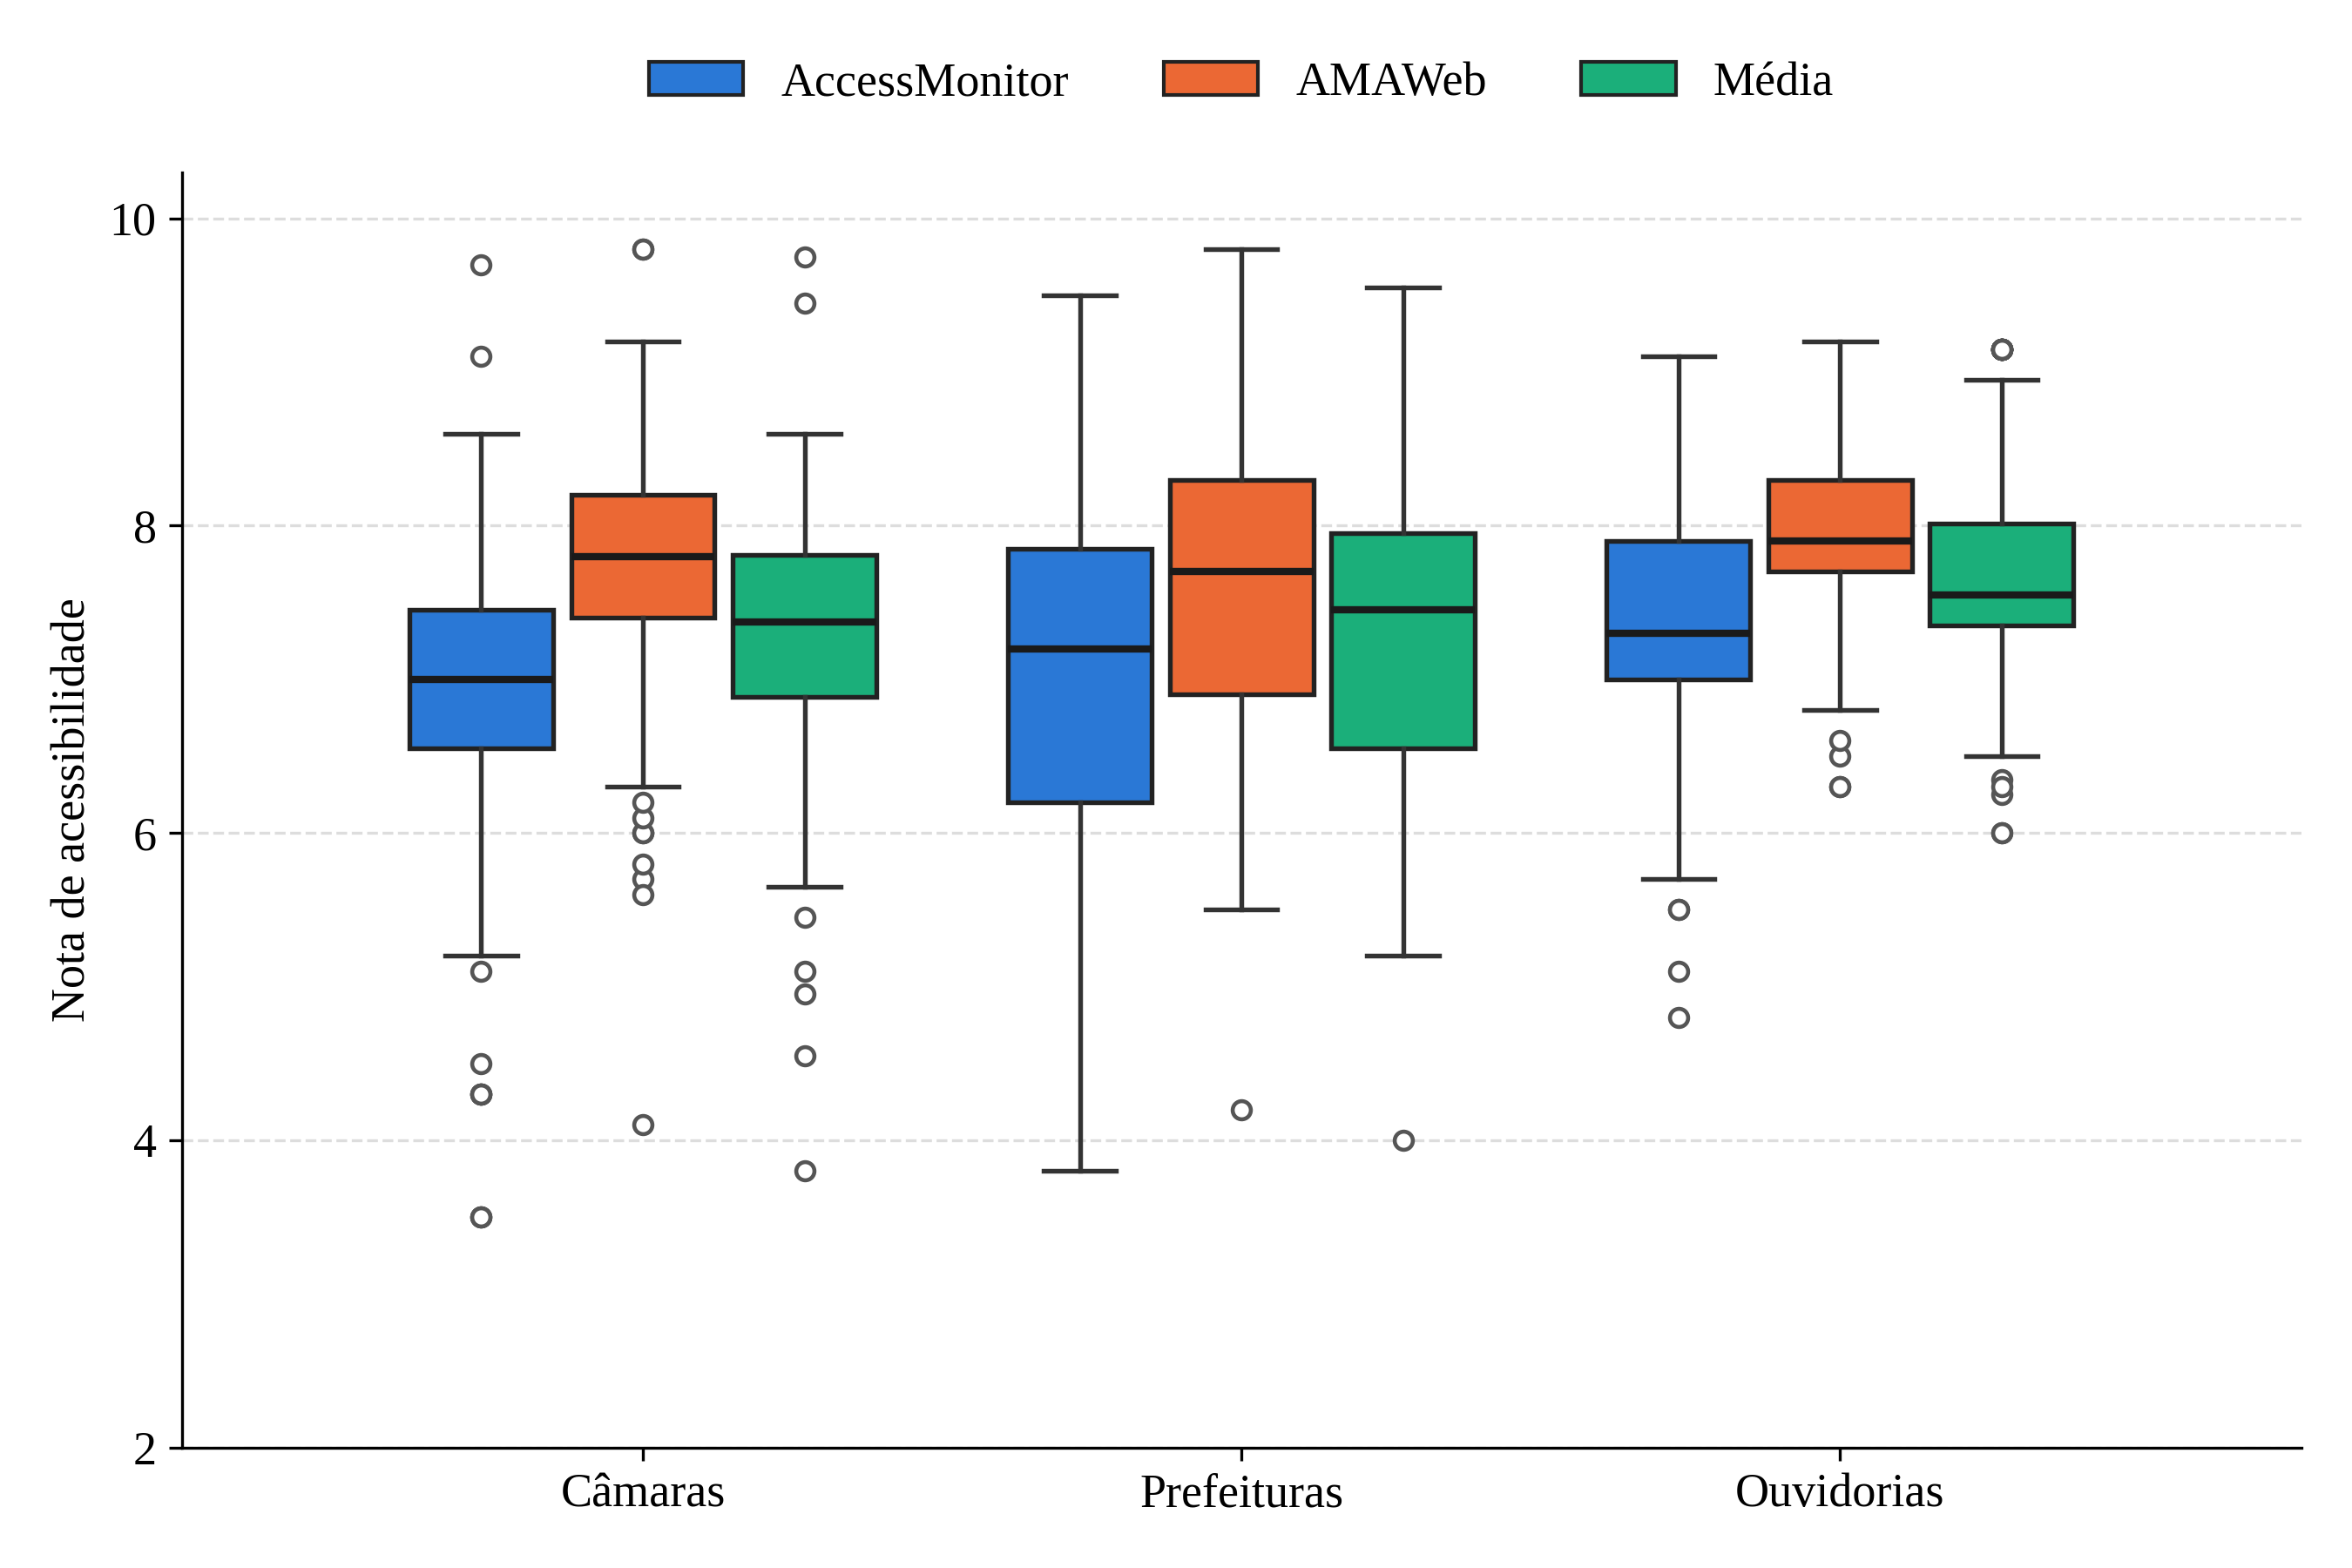
\includegraphics[width=0.9\linewidth]{images/boxplot_egov_artigo.png}
\caption{Distribuição das notas de acessibilidade por ambiente e ferramenta. A série Média corresponde à média entre as notas das duas ferramentas.}
\label{fig:boxplot}
\end{figure}

\begin{table}[ht]
\centering
\caption{Estatística descritiva das notas de acessibilidade, por ambiente e ferramenta}
\label{tab:descritiva}
\footnotesize
\setlength{\tabcolsep}{4pt}
\begin{tabular}{lrrrrrr}
\toprule
 & \multicolumn{2}{c}{\textbf{Prefeitura}} & \multicolumn{2}{c}{\textbf{Câmara}} & \multicolumn{2}{c}{\textbf{Ouvidoria}} \\
\cmidrule(lr){2-3}\cmidrule(lr){4-5}\cmidrule(lr){6-7}
\textbf{Medida} & \textbf{AMAWeb} & \textbf{AccessM.} & \textbf{AMAWeb} & \textbf{AccessM.} & \textbf{AMAWeb} & \textbf{AccessM.} \\
\midrule
$n$                  &  117 &  123 &  100 &  107 &  101 &  116 \\
Média                & 7,65 & 7,01 & 7,68 & 6,89 & 7,98 & 7,48 \\
Mediana              & 7,70 & 7,20 & 7,80 & 7,00 & 7,90 & 7,30 \\
Desvio-padrão        & 1,00 & 1,22 & 0,88 & 1,15 & 0,68 & 0,91 \\
Mínimo               & 4,20 & 3,80 & 4,10 & 3,50 & 6,30 & 4,80 \\
Máximo               & 9,80 & 9,50 & 9,80 & 9,70 & 9,20 & 9,10 \\
\midrule
\multicolumn{7}{l}{\textit{Distribuição por faixa de nota (\%)}} \\
Abaixo de 5,0        &  0,9 &  6,5 &  1,0 &  7,5 &  0,0 &  0,9 \\
5,0 a 6,9            & 24,8 & 33,3 & 14,0 & 39,3 &  5,0 & 12,1 \\
7,0 a 8,9            & 65,0 & 54,5 & 82,0 & 51,4 & 79,2 & 75,0 \\
9,0 ou mais          &  9,4 &  5,7 &  3,0 &  1,9 & 15,8 & 12,1 \\
\bottomrule
\end{tabular}
\end{table}

A maior parte das páginas ficou na faixa de 7,0 a 8,9 pontos em todos os ambientes. A proporção de páginas com nota igual ou superior a 9,0 foi pequena, sobretudo nas câmaras (3,0\% no AMAWeb e 1,9\% no AccessMonitor), enquanto as notas abaixo de 7,0 foram mais frequentes nos portais das prefeituras e das câmaras avaliados pelo AccessMonitor (39,8\% e 46,8\%, respectivamente).

A Tabela~\ref{tab:erros} lista as práticas classificadas como não aceitáveis com maior frequência no AMAWeb. O contraste de cor insuficiente e os links sem nome acessível foram os problemas mais comuns nos três ambientes. Os perfis de erro, contudo, diferem. Nos portais das prefeituras, destacam-se problemas de marcação, como atributos \texttt{id} repetidos (65,0\%). Nos portais das câmaras, sobressaem os links sem nome acessível (82,0\%) e a ausência ou duplicação do cabeçalho \texttt{h1} (74,0\%). Nas ouvidorias, predominam falhas associadas à navegação por teclado, como a ausência de mecanismo para saltar ao conteúdo principal e a remoção do foco por JavaScript (75,2\% cada). Essas falhas são indícios de barreiras para quem usa teclado ou leitor de tela ao preencher um formulário; a confirmação do impacto efetivo exige inspeção manual e testes com usuários. O idioma principal marcado incorretamente aparece em 55,4\% das ouvidorias, contra 5,1\% dos portais das prefeituras e 3,0\% dos das câmaras, o que é compatível com a replicação de uma mesma plataforma em diversos municípios. O AccessMonitor reproduziu o padrão geral: contraste insuficiente em 74,8\% dos portais das prefeituras, 72,9\% dos das câmaras e 68,1\% das ouvidorias, e ausência de link para saltar ao conteúdo em 69,0\% das ouvidorias.

\begin{table}[ht]
\centering
\caption{Práticas classificadas como não aceitáveis com maior frequência no AMAWeb}
\label{tab:erros}
\footnotesize
\setlength{\tabcolsep}{3pt}
\begin{tabular}{lccrrr}
\toprule
 & & & \multicolumn{3}{c}{\textbf{Páginas com o erro (\%)}} \\
\cmidrule(lr){4-6}
\textbf{Erro} & \textbf{Critério} & \textbf{Nível} & \textbf{Prefeituras} & \textbf{Câmaras} & \textbf{Ouvidorias} \\
 & \textbf{WCAG} & & ($n=117$) & ($n=100$) & ($n=101$) \\
\midrule
Contraste de cor insuficiente                     & 1.4.3  & AA  & 84,6 & 78,0 & 73,3 \\
Links sem nome acessível                          & 4.1.2  & A   & 76,1 & 82,0 & 58,4 \\
Atributos \texttt{id} repetidos                   & 4.1.1  & A   & 65,0 & 45,0 & 15,8 \\
Links de imagem sem texto alternativo             & 2.4.4  & A   & 59,0 & 58,0 & 56,4 \\
Ausência de \texttt{h1} ou \texttt{h1} duplicado  & 1.3.1  & A   & 51,3 & 74,0 & 57,4 \\
Sem link para saltar ao conteúdo                  & 2.4.1  & A   & 46,2 & 45,0 & 75,2 \\
Foco removido por JavaScript                      & 2.4.7  & AA  & 41,0 & 16,0 & 75,2 \\
Hierarquia de cabeçalhos violada                  & 2.4.10 & AAA & 40,2 & 37,0 & 67,3 \\
Idioma principal marcado incorretamente           & 3.1.1  & A   &  5,1 &  3,0 & 55,4 \\
\bottomrule
\end{tabular}
\end{table}

\subsection{Consistência entre os ambientes do mesmo município (QP2)}

A Tabela~\ref{tab:pareado} compara as notas da prefeitura com as da ouvidoria e as da câmara, nos municípios com os dois ambientes avaliados na mesma ferramenta. A ouvidoria obteve nota maior que o portal da prefeitura em 53 dos 96 municípios no AMAWeb e em 50 dos 109 no AccessMonitor, com diferenças médias de $-0{,}38$ e $-0{,}43$ ponto. A diferença foi estatisticamente significativa no AMAWeb, mas não no AccessMonitor. Na comparação com a câmara, as médias foram praticamente iguais, e as diferenças não foram significativas em nenhuma ferramenta.

\begin{table}[ht]
\centering
\caption{Comparação pareada entre o portal da prefeitura e os demais ambientes do mesmo município}
\label{tab:pareado}
\small
\setlength{\tabcolsep}{4pt}
\begin{tabular}{lrrrr}
\toprule
 & \multicolumn{2}{c}{\textbf{Prefeitura $\times$ Ouvidoria}} & \multicolumn{2}{c}{\textbf{Prefeitura $\times$ Câmara}} \\
\cmidrule(lr){2-3}\cmidrule(lr){4-5}
\textbf{Medida} & \textbf{AMAWeb} & \textbf{AccessM.} & \textbf{AMAWeb} & \textbf{AccessM.} \\
\midrule
Municípios comparados                          & 96 & 109 & 93 & 99 \\
Outro ambiente com nota maior                  & 53 & 50 & 45 & 43 \\
Outro ambiente com nota menor                  & 38 & 52 & 45 & 52 \\
Notas iguais                                   & 5 & 7 & 3 & 4 \\
Diferença média (prefeitura $-$ outro)         & $-$0,38 & $-$0,43 & 0,00 & 0,17 \\
Diferença absoluta média                       & 0,92 & 1,17 & 0,98 & 1,19 \\
Teste de Wilcoxon ($p$)                        & 0,007 & 0,094 & 0,937 & 0,287 \\
\bottomrule
\end{tabular}
\end{table}

A diferença absoluta média, no entanto, foi próxima de um ponto nas duas comparações e nas duas ferramentas. Isso significa que, mesmo quando as médias gerais são semelhantes, as notas de um mesmo município variam de forma relevante entre os ambientes, ora a favor de um, ora de outro. A nota do portal da prefeitura, portanto, não representa a da ouvidoria nem a do portal da câmara, e cada ambiente precisa ser avaliado separadamente.

\subsection{Tipos de solução de ouvidoria (QP3)}

A Tabela~\ref{tab:tipos} apresenta a frequência de cada tipo de solução de ouvidoria, as notas médias dos formulários confirmados e a diferença em relação ao portal da prefeitura.

\begin{table}[ht]
\centering
\caption{Tipos de solução de ouvidoria, notas médias da ouvidoria e diferença média prefeitura $-$ ouvidoria, por ferramenta}
\label{tab:tipos}
\footnotesize
\setlength{\tabcolsep}{3pt}
\begin{tabular}{lrrrrrr}
\toprule
 & & & \multicolumn{2}{c}{\textbf{Nota da ouvidoria ($n$)}} & \multicolumn{2}{c}{\textbf{Diferença média (pares)}} \\
\cmidrule(lr){4-5}\cmidrule(lr){6-7}
\textbf{Tipo} & \textbf{Municípios} & \textbf{\%} & \textbf{AMAWeb} & \textbf{AccessM.} & \textbf{AMAWeb} & \textbf{AccessM.} \\
\midrule
Integrada ao portal  & 37 & 26,1 & 7,63 (15) & 7,11 (28) & $-$0,09 (13) &    0,08 (23) \\
Sistema próprio      & 59 & 41,5 & 7,83 (55) & 7,24 (57) & $-$0,02 (53) &    0,17 (56) \\
Terceirizada         & 36 & 25,4 & 8,54 (24) & 8,25 (24) & $-$1,30 (23) & $-$2,07 (23) \\
Fala.BR              &  9 &  6,3 & 8,00 (7)  & 8,30 (7)  & $-$0,57 (7)  & $-$1,46 (7) \\
Indisponível         &  1 &  0,7 &  ---      &  ---      &     ---      &     --- \\
\midrule
\textbf{Total}       & \textbf{142} & \textbf{100} & & & & \\
\bottomrule
\multicolumn{7}{p{0.95\linewidth}}{\footnotesize Notas calculadas apenas sobre os formulários confirmados com avaliação válida em cada ferramenta. Diferença negativa indica ouvidoria com nota maior que o portal da prefeitura.}
\end{tabular}
\end{table}

Os sistemas próprios em domínio ou subdomínio distinto são o tipo mais frequente (41,5\%), e 54 dos 59 seguem o mesmo padrão de endereço (\texttt{ouvidoria.<município>.mt.gov.br/Manifestacao/}). Isso sugere que parte dos canais classificados como próprios é, na verdade, uma mesma solução replicada entre municípios, possivelmente fornecida por uma única empresa e hospedada sob o domínio da prefeitura. O mesmo ocorre entre as terceirizadas, que se concentram em poucos fornecedores. As integradas ao portal respondem por 26,1\%, as terceirizadas por 25,4\%, e 9 municípios (6,3\%) direcionam o cidadão ao Fala.BR.

Nas ouvidorias integradas ao portal e nos sistemas próprios, a diferença média em relação ao portal da prefeitura é próxima de zero. Já as ouvidorias terceirizadas obtiveram notas mais altas que o respectivo portal em 18 dos 23 municípios comparados, nas duas ferramentas, com diferenças médias de 1,30 e 2,07 pontos. Os dados mostram uma associação entre o tipo de ouvidoria e a diferença de notas, mas não permitem atribuí-la ao fornecedor ou à política de acessibilidade do município. No caso do Fala.BR, os municípios avaliados utilizam a mesma página de registro; por isso, suas notas não representam implementações independentes.

\subsection{Relação com porte populacional e indicadores socioeconômicos (QP4)}

Antes das análises com a nota consolidada, verificou-se a concordância entre as ferramentas. A correlação entre as notas do AMAWeb e do AccessMonitor para uma mesma página foi de 0,91 nos portais das prefeituras, 0,79 nos das câmaras e 0,71 nas ouvidorias, e a diferença entre as ferramentas foi aproximadamente constante (entre 0,49 e 0,85 ponto, conforme o ambiente). Nessas condições, a média das duas notas preserva, em grande parte, a ordem dos municípios, o que foi confirmado no ranqueamento (Seção~\ref{sec:ranking}).

A Tabela~\ref{tab:correlacao} apresenta os coeficientes de correlação de Spearman entre as notas consolidadas e os indicadores municipais. A única associação significativa foi a correlação negativa fraca entre o PIB \textit{per capita} e a nota dos portais das prefeituras ($\rho = -0{,}268$; $p = 0{,}004$). Nas ouvidorias, a correlação com a população foi positiva e fraca, mas não significativa ($\rho = 0{,}194$; $p = 0{,}053$). Nos portais das câmaras, nenhuma associação foi significativa.

\begin{table}[ht]
\centering
\caption{Correlação de Spearman ($\rho$) entre as notas consolidadas e os indicadores municipais}
\label{tab:correlacao}
\small
\begin{tabular}{lrrr}
\toprule
\textbf{Indicador} & \textbf{Prefeitura} & \textbf{Câmara} & \textbf{Ouvidoria} \\
\midrule
População (IBGE, 2026)         & $-$0,155   &    0,029 &    0,194 \\
PIB \textit{per capita} (2023) & $-$0,268** & $-$0,038 & $-$0,041 \\
IDHM (2010)                    & $-$0,171   & $-$0,042 & $-$0,025 \\
\midrule
$n$                            & 117 & 100 & 100 \\
\bottomrule
\multicolumn{4}{l}{\footnotesize * $p < 0{,}05$; ** $p < 0{,}01$.}
\end{tabular}
\end{table}

A Tabela~\ref{tab:faixas} apresenta as médias por faixa populacional nos 75 municípios da base do ranqueamento. As notas não cresceram de forma consistente com o porte populacional. Nas ouvidorias, a maior média ocorreu entre os municípios acima de 50 mil habitantes, mas esse estrato contém apenas oito observações.

\begin{table}[ht]
\centering
\caption{Notas médias consolidadas por faixa populacional}
\label{tab:faixas}
\small
\begin{tabular}{lrrrrr}
\toprule
\textbf{Faixa populacional} & \textbf{$n$} & \textbf{Prefeitura} & \textbf{Câmara} & \textbf{Ouvidoria} & \textbf{Média} \\
\midrule
Até 10 mil habitantes      & 27 & 7,57 & 7,14 & 7,76 & 7,49 \\
De 10 a 50 mil habitantes  & 40 & 7,09 & 7,36 & 7,78 & 7,41 \\
Acima de 50 mil habitantes &  8 & 7,22 & 7,31 & 8,21 & 7,58 \\
\bottomrule
\end{tabular}
\end{table}

\subsection{Ranqueamento dos municípios}
\label{sec:ranking}

O ranqueamento foi calculado para os 75 municípios com os três ambientes avaliados pelas duas ferramentas. Para cada ambiente, calculou-se a nota consolidada, e a nota final corresponde à média simples das três notas consolidadas. Em caso de empate, adotou-se a ordem alfabética. A amplitude corresponde à diferença entre a maior e a menor nota consolidada do município. As Tabelas~\ref{tab:ranking} e~\ref{tab:ranking_ultimos} apresentam os dez municípios mais bem e os dez mais mal posicionados; a lista completa está disponível em XX.

\begin{table}[ht]
\centering
\caption{Dez municípios com maiores médias consolidadas de acessibilidade ($n = 75$)}
\label{tab:ranking}
\footnotesize
\setlength{\tabcolsep}{4pt}
\begin{tabular}{rlrrrrr}
\toprule
\textbf{\#} & \textbf{Município} & \textbf{Prefeitura} & \textbf{Câmara} & \textbf{Ouvidoria} & \textbf{Média} & \textbf{Amplitude} \\
\midrule
1  & Nossa Senhora do Livramento      & 8,95 & 9,45 & 7,35 & 8,58 & 2,10 \\
2  & Conquista d'Oeste                & 9,30 & 7,50 & 8,65 & 8,48 & 1,80 \\
3  & Sinop                            & 9,55 & 8,30 & 7,50 & 8,45 & 2,05 \\
4  & Cuiabá                           & 8,00 & 9,75 & 7,00 & 8,25 & 2,75 \\
5  & Porto Esperidião                 & 8,75 & 8,60 & 7,35 & 8,23 & 1,40 \\
6  & Vila Rica                        & 8,40 & 8,45 & 7,55 & 8,13 & 0,90 \\
7  & Vila Bela da Santíssima Trindade & 7,90 & 8,50 & 7,90 & 8,10 & 0,60 \\
8  & Rondolândia                      & 7,80 & 7,75 & 8,65 & 8,07 & 0,90 \\
9  & Itanhangá                        & 6,80 & 8,20 & 9,15 & 8,05 & 2,35 \\
10 & Tapurah                          & 7,55 & 7,25 & 9,15 & 7,98 & 1,90 \\
\bottomrule
\end{tabular}
\end{table}

\begin{table}[ht]
\centering
\caption{Dez municípios com menores médias consolidadas de acessibilidade ($n = 75$)}
\label{tab:ranking_ultimos}
\footnotesize
\setlength{\tabcolsep}{4pt}
\begin{tabular}{rlrrrrr}
\toprule
\textbf{\#} & \textbf{Município} & \textbf{Prefeitura} & \textbf{Câmara} & \textbf{Ouvidoria} & \textbf{Média} & \textbf{Amplitude} \\
\midrule
66 & Marcelândia             & 5,50 & 7,75 & 7,40 & 6,88 & 2,25 \\
67 & Santa Rita do Trivelato & 5,40 & 6,40 & 8,85 & 6,88 & 3,45 \\
68 & Matupá                  & 6,55 & 7,70 & 6,35 & 6,87 & 1,35 \\
69 & Pedra Preta             & 5,75 & 7,05 & 7,55 & 6,78 & 1,80 \\
70 & São Pedro da Cipa       & 8,30 & 5,45 & 6,30 & 6,68 & 2,85 \\
71 & Nova Marilândia         & 7,90 & 4,55 & 7,40 & 6,62 & 3,35 \\
72 & Nortelândia             & 7,50 & 4,95 & 7,35 & 6,60 & 2,55 \\
73 & Querência               & 5,80 & 5,95 & 7,35 & 6,37 & 1,55 \\
74 & Itiquira                & 6,45 & 6,55 & 6,00 & 6,33 & 0,55 \\
75 & Arenápolis              & 6,05 & 3,80 & 6,95 & 5,60 & 3,15 \\
\bottomrule
\end{tabular}
\end{table}

O ranqueamento consolidado mostrou-se robusto. Sua correlação com o ranqueamento feito apenas com o AccessMonitor foi de 0,95, e com o feito apenas com o AMAWeb, de 0,87; com notas padronizadas por escore-z, foi de 0,97. Oito dos dez primeiros coincidem com os dos ranqueamentos por ferramenta, e nove com os do ranqueamento padronizado. O ranqueamento também reforça a variação entre os ambientes do mesmo município: a amplitude média foi de 1,57 ponto, e 25 dos 75 municípios tiveram diferença de 2 pontos ou mais entre o melhor e o pior ambiente. Mesmo entre os mais bem posicionados há municípios com um ambiente bem abaixo dos demais, como Cuiabá, cuja ouvidoria obteve 7,00, enquanto o portal da câmara obteve 9,75.

\subsection{Discussão}

À luz do Modelo de Sucesso de SI de DeLone e McLean~\cite{delone1992,delone2003}, os resultados indicam que a qualidade do sistema, operacionalizada pela conformidade com as diretrizes de acessibilidade, não é homogênea entre os canais de um mesmo município. Como a ouvidoria e o portal da câmara costumam ser acessados a partir do portal da prefeitura, falhas em qualquer um desses ambientes podem comprometer o percurso do cidadão e, com isso, o uso e a satisfação com o serviço. Esse achado indica, para o contexto municipal, o limite das avaliações restritas à página inicial~\cite{valtolina2022,eres,franca2025}.

O contraste insuficiente e a falta de nomes acessíveis em links, presentes nos três ambientes, são falhas de correção relativamente simples, que dependem mais de diretrizes de projeto do que de mudanças estruturais nos sistemas. A concentração de falhas associadas à navegação por teclado nas ouvidorias merece atenção, pois esses canais existem justamente para receber manifestações, inclusive sobre a falta de acessibilidade~\cite{lei13460}. A localização dos canais também revelou que 14 municípios não levam o cidadão diretamente a um formulário, mas a portais intermediários ou a páginas de contato.

As correlações fracas com os indicadores socioeconômicos são compatíveis com o estudo dos condados norte-americanos, no qual o orçamento teve efeito apenas marginal sobre a acessibilidade~\cite{bai2021}. A correlação negativa entre o PIB \textit{per capita} e a nota dos portais das prefeituras, embora fraca, indica que maior capacidade econômica não se traduz, por si só, em portais mais acessíveis. O desempenho das ouvidorias terceirizadas e a replicação de uma mesma solução em dezenas de municípios levantam a hipótese de que a acessibilidade dependa mais das soluções contratadas e de sua gestão do que do porte do município. Essa hipótese é coerente com os achados sobre a terceirização da responsabilidade pelos testes de acessibilidade~\cite{nunes2025} e sobre o papel da supervisão e da revisão periódica dos sítios~\cite{frandell2026}, mas as decisões de contratação e de gestão não foram medidas neste estudo e devem ser investigadas diretamente em trabalhos futuros.


\section{Considerações finais}
\label{sec:consideracoes}

Este estudo abrangeu os 142 municípios de Mato Grosso e avaliou a acessibilidade digital dos portais das prefeituras, dos portais das câmaras municipais e dos canais eletrônicos de ouvidoria, com duas ferramentas automatizadas baseadas nas WCAG 2.1, o AMAWeb e o AccessMonitor. O formulário de ouvidoria foi confirmado em 127 municípios, e os três ambientes tiveram avaliação válida em 88 municípios com ao menos uma ferramenta e em 75 com as duas.

Em relação à QP1, as ouvidorias obtiveram as maiores médias e a menor dispersão, e a maior parte das páginas dos três ambientes ficou entre 7,0 e 8,9 pontos. O contraste insuficiente e os links sem nome acessível foram os problemas mais comuns, e as ouvidorias concentraram falhas associadas à navegação por teclado e ao foco, que são indícios de barreiras justamente para quem usa teclado ou leitor de tela ao registrar uma manifestação. Em relação à QP2, a nota do portal da prefeitura não representou a dos demais ambientes: a diferença absoluta média entre ambientes do mesmo município foi próxima de um ponto, tanto em relação à ouvidoria quanto à câmara. Em relação à QP3, as ouvidorias terceirizadas obtiveram notas superiores às dos respectivos portais em 18 dos 23 municípios comparados, e a replicação de uma mesma solução em dezenas de municípios indica que parte dos resultados reflete a plataforma adotada. Em relação à QP4, a única associação significativa foi a correlação negativa fraca entre o PIB \textit{per capita} e a nota dos portais das prefeituras, e os dados não sustentam a interpretação de que municípios maiores ou com melhores indicadores socioeconômicos ofereçam páginas mais acessíveis.

Os resultados mostram também que a existência de um canal eletrônico não assegura condições adequadas de acesso. Em 14 municípios, o caminho encontrado leva a um portal intermediário ou a uma página de contato, e não a um formulário de manifestação. Além disso, bloqueios por serviços de proteção, erros internos das ferramentas, esgotamentos de tempo, falhas de DNS e certificados inválidos reduziram a cobertura da coleta; essas ocorrências podem igualmente dificultar o acesso do cidadão aos serviços públicos digitais.

Quanto às \textit{Contributions and Impact to IS area}, o trabalho oferece um diagnóstico inédito da acessibilidade digital municipal em Mato Grosso, que abrange todos os municípios do estado, mostra que cada canal do município precisa ser avaliado separadamente e fornece um procedimento de coleta replicável e uma linha de base para o acompanhamento do governo digital no estado. À luz do Modelo de Sucesso de SI de DeLone e McLean, os resultados evidenciam que a qualidade do sistema, condição para o uso e a satisfação do cidadão, ainda apresenta fragilidades nos canais municipais, inclusive naqueles destinados à participação. Como implicação prática, recomenda-se que as administrações municipais incluam requisitos de acessibilidade nos processos de contratação e atualização de portais e sistemas de ouvidoria, mantenham rotinas periódicas de avaliação e exijam a correção das falhas identificadas nos componentes compartilhados.

O estudo tem limitações. As notas automatizadas sintetizam apenas os critérios verificáveis pelas ferramentas e não substituem inspeções manuais, testes com tecnologias assistivas ou a participação de pessoas com deficiência. Avaliou-se uma única página de cada ambiente, e a pesquisa representa um recorte temporal, pois as páginas governamentais são alteradas continuamente. O uso do HTML baixado como contingência não reproduz integralmente conteúdos gerados por \textit{scripts} ou interações dinâmicas. A situação de parte das ouvidorias sem avaliação válida foi definida a partir dos registros de falha da coleta e de uma verificação manual posterior. Além disso, o ranqueamento considerou apenas os 75 municípios com os três ambientes avaliados pelas duas ferramentas. Essa decisão garante que todos sejam comparados na mesma base, já que o AMAWeb atribui notas sistematicamente mais altas que o AccessMonitor, mas exclui do ranqueamento 67 municípios, em geral por falhas de uma das ferramentas, por ambientes não avaliados ou por ouvidorias sem formulário confirmado. A nota consolidada também combina ferramentas com escalas que não são equivalentes; embora o ranqueamento tenha se mostrado robusto à escolha da ferramenta e à padronização das notas, ele deve ser compreendido como instrumento diagnóstico e linha de base para acompanhamento, e não como certificação de conformidade.

Para trabalhos futuros, propõe-se complementar a avaliação automatizada com inspeções manuais e testes com usuários com deficiência, avaliar outras páginas de cada ambiente, investigar diretamente o papel das decisões de contratação e de gestão das soluções digitais, acompanhar longitudinalmente a evolução dos municípios e ampliar a análise para outros serviços públicos digitais. Dessa forma, o diagnóstico pode apoiar políticas de governo digital orientadas não apenas à disponibilidade dos serviços, mas também à sua utilização efetiva, autônoma e equitativa por toda a população.


\section*{Declaração de uso de inteligência artificial}

Durante a elaboração deste trabalho, os autores utilizaram o assistente de inteligência artificial Claude (Anthropic) para apoiar a elaboração do código da figura que representa o processo metodológico (Figura~\ref{fig:metodologia}), a revisão textual do manuscrito e a tradução do resumo para o inglês. Todo o conteúdo gerado com apoio da ferramenta foi revisado e validado pelos autores, que assumem integral responsabilidade pelo texto, pelos dados e pelas conclusões apresentados.

\bibliographystyle{sbc}
\bibliography{sbc-template}

\end{document}